\documentclass{memoir}
\usepackage[utf8]{inputenc}
\usepackage[ukrainian]{babel}
\usepackage{enumitem}
\usepackage{tikz}
\usepackage{listings}
\usepackage{amsmath}

\lefthyphenmin=1
\hyphenpenalty=100
\tolerance=4000
\emergencystretch=1em
\hfuzz=2pt
\vfuzz=2pt

\lstset{
    basicstyle=\ttfamily\footnotesize,
    breaklines=true,
    keywordstyle=\bfseries,
    inputencoding=utf8,
    extendedchars=true,
    showstringspaces=false
}

\setlist[itemize]{noitemsep}
\setlist[enumerate]{noitemsep}

\begin{document}

\begin{center}
    \vspace*{3cm}
    {\Huge \textbf{Компілятор PL/IL}}\\[0.5cm]
    {\Large Проектування та розробка}\\[1cm]
    {\normalsize Версія 2004.06.01}\\[1cm]
    {\normalsize Максим Е. Сохацький (\texttt{maxim.sokhatsky@gmail.com})}\\
    {\normalsize Олег В. Смірнов (\texttt{oleg.smirnov@gmail.com})}\\[0.5cm]
    \vspace{5cm}
    {\normalsize Київський Політехнічний Інститут}\\
    {\normalsize 2004}
\end{center}

\newpage
\tableofcontents

\newpage

\chapter{Вступ}
\section{Поставлені цілі}
Основне завдання, поставлене перед розробниками цього проєкту,
полягало в реалізації мови програмування PL/1 для єдиної мовної
середовища Microsoft Common Language Runtime (CLR), з підтримкою
Common Intermediate Language (CIL) – об’єктно-орієнтованого стекового
асемблера для віртуальної машини CLR. Єдина мовна інфраструктура (Common
Language Infrastructure) разом із системою класів Microsoft .NET Framework
є найсучаснішим способом створення застосунків для операційних систем Microsoft.

\section{Єдине мовне середовище Microsoft}
Завдяки Єдиній системі типів (Common Type System, CTS) CLR забезпечує можливість
використовувати однаковий спосіб взаємодії застосунків, написаних різними мовами.
Такі технології пізнього зв’язування та компонентні моделі, як COM і ActiveX,
що використовують домовленості щодо структур об’єктів, більше не потрібні.
На сьогодні існує майже повний спектр імперативних мов програмування,
які використовують CLR як носій об’єктного коду: Pascal, C, Java, Python,
Perl, Cobol, Fortran. Реалізації бракує лише однієї з найстаріших і
найпотужніших мов – PL/1, яку автори цієї роботи вирішили відродити
в об’єктно-орієнтованій парадигмі.

\section{Об’єктно-орієнтований PL/1}
PL/1 досі залишається однією з найпотужніших мов програмування завдяки своїй здатності підставляти константи, описані в програмі, як виконувану програму. Це одна з багатьох переваг PL/1, яка легко реалізується в середовищі CLR.

\section{Особливості PL/IL}
Компілятор PL/IL, який використовує CLR і .NET Framework як хост, має низку особливостей:
\begin{itemize}
    \item Компіляція EXE та DLL збірок CLR.
    \item Використання класів .NET Framework.
    \item Єдина система типів CTS.
    \item Генерація лістингу програми на IL.
    \item Використання Reflection для підставок.
    \item Структурна обробка винятків.
    \item Вбудований контроль типів.
\end{itemize}
Завдяки цим можливостям можна створювати навіть вебсервіси, використовуючи PL/IL. Крім того, можна використовувати збірки, написані іншими мовами, що підтримують CLI, наприклад C\# або Visual Basic .NET, через лінкування або динамічне завантаження. Діалект PL/IL максимально наближений до PL/M – оптимізованої версії PL/1 для мікроконтролерів.

\section{Перспективи}
На відміну від віртуальних машин Java, CLR має специфікацію на єдину систему типів, спільну для всіх мов CLI. Крім того, на відміну від Java, усі специфікації на ці технології затверджені ECMA, що гарантує сумісність майбутніх кросплатформних реалізацій CLR, таких як MONO.

\chapter{Теоретичні відомості}
\section{Структура компілятора}
Основні етапи, які проходить компілятор, включають:
\begin{itemize}
    \item Лексичний аналіз.
    \item Синтаксичний аналіз.
    \item Контекстний аналіз.
    \item Машинно-незалежний оптимізатор.
    \item Генератор коду.
    \item Оптимізатор коду.
\end{itemize}
Інформація, необхідна на етапах компіляції, класифікується так:
\begin{itemize}
    \item Вихідний текст програми.
    \item Таблиця термінальних символів мови.
    \item Лексична згортка.
    \item Правила граматики.
    \item Дерево виведення.
    \item Абстрактна програма.
    \item Проміжний код.
    \item Об’єктний код.
\end{itemize}

\section{Теоретичні питання}
Можна виділити такі теми для освоєння теорії побудови програмних систем:
\begin{enumerate}
    \item Лексичний аналіз.
    \item Синтаксичний аналіз.
    \item Синтаксично керована трансляція.
    \item Система типів і середовище виконання.
    \item Генерація проміжного коду.
    \item Генерація об’єктного коду.
\end{enumerate}

\section{Основні методи синтаксичного аналізу}
\subsection{Нисхідний аналіз}
Усунувши з граматики ліву рекурсію, можна ефективно реалізувати аналіз методом рекурсивного спуску без відкатів. Також можна використовувати табличні методи аналізу без відкатів для граматик із усунутою лівою рекурсією. Автори обрали нисхідний аналіз, оскільки LL-граматика виглядає більш естетично. Метод рекурсивного спуску без відкатів полегшує розуміння компілятора іншими розробниками, підвищує ступінь спільної розробки та є більш гнучким і розширюваним порівняно з табличними методами.

\subsection{Висхідний аналіз}
Для висхідного аналізу існують алгоритми типу «перенесення-згортка», а також генератори аналізаторів LR і LALR граматик.

\subsection{Метод рекурсивного спуску}
Цей метод добре підходить для простих LL(1)-граматик, хоча може використовуватися і для синтаксичних аналізаторів із відкатами. Синтаксичний аналізатор будується так, що для кожного нетермінала визначається одна рекурсивна процедура. Правила граматики перетворюються для однозначного визначення альтернатив і цілеспрямованого виведення. Наприклад, якщо є правила:
\[
A \to \alpha \, t_1 \, \beta \mid \alpha \, t_2 \, \gamma \, ; \, t_1, t_2 \in \Sigma \, ; \, \alpha, \beta, \gamma - \text{довільні ланцюжки},
\]
вони перетворюються до виду:
\[
A \to \alpha \, ( \, t_1 \, \beta \mid t_2 \, \gamma \, ),
\]
де \( ( \dots ) \) – скобки факторизації.

Правила виду:
\[
A \to \alpha \mid A \, t \, \beta,
\]
де \( t \in \Sigma \), \( \alpha, \beta \in (N \cup \Sigma)^* \), перетворюються до:
\[
A \to \alpha \, \{ \, t \, \beta \, \},
\]
де \( \{ \dots \} \) – рекурсивна частина.

Правила виду:
\[
A \to \alpha \mid \alpha \, t \, \beta,
\]
записуються як:
\[
A \to \alpha \, [ \, t \, \beta \, ],
\]
де \( [ \dots ] \) – необов’язкова конструкція.

Приклад граматики:
\begin{align*}
A_1 &\to A_2 \, := \, A_3 \mid \text{if} \, A_3 \, \text{then} \, A_1 \mid \text{if} \, A_3 \, \text{then} \, A_1 \, \text{else} \, A_1 \\
A_2 &\to i \mid i \, ( \, A_3 \, ) \\
A_3 &\to A_4 \mid A_3 \, + \, A_4 \\
A_4 &\to A_5 \mid A_4 \, * \, A_5 \\
A_5 &\to A_2 \mid ( \, A_3 \, )
\end{align*}
Для процедур правила переписуються так:
\begin{align*}
A_1 &\to A_2 \, := \, A_3 \mid \text{if} \, A_3 \, \text{then} \, A_1 \, [ \, \text{else} \, A_1 \, ] \\
A_2 &\to i \, [ \, ( \, A_3 \, ) \, ] \\
A_3 &\to A_4 \, \{ \, + \, A_4 \, \} \\
A_4 &\to A_5 \, \{ \, * \, A_5 \, \} \\
A_5 &\to A_2 \mid ( \, A_3 \, )
\end{align*}

Приклад процедури для \( A_1 \):
\begin{lstlisting}
int next;
void A1() {
    if (next == IF) {
        scan();
        A3();
        if (next != THEN) error();
        else {
            scan();
            A1();
            if (next == ELSE) {
                scan();
                A1();
            }
        }
    } else {
        A2();
        if (next != AS) error();
        else {
            scan();
            A3();
        }
    }
}
\end{lstlisting}

\newpage
\begin{lstlisting}
A2()
{
    if (next != ID) error(); else {
        scan();
        if (next == LP) {
            scan();
            A3();
            if (next != RP) error(); else scan();
        }
     }
}

A3()
{
    A4();
    while (next == PLUS) { scan (); A4(); }
}
\end{lstlisting}

\chapter{Компілятор PL/IL}
\section{Історія}
PL/IL – це підмножина мови PL/1, створеної IBM, яка активно використовувалася в 60-х роках. У країнах колишнього СРСР ця мова застосовувалася в машинах ЄС ЕОМ, що було логічно, оскільки ЄС ЕОМ була аналогом обчислювальних комплексів IBM System/360. Символ «/» характерний для назв продуктів IBM, наприклад, System/360, ES/9000, RS/6000, AS/400, PS/2, OS/2, PL/1.

Від часу створення PL/1 було реалізовано багато мов із повністю або частково сумісним синтаксисом. Компанія Intel розробила PL/M – підмножину PL/1 для мікроконтролерів, що відображено в «M» у назві. PL/IL є підмножиною PL/M, яка, у свою чергу, є підмножиною PL/1. Наразі підмножина PL/SQL використовується в системах управління базами даних Oracle. Багато компаній, що займаються підтримкою старих мейнфреймів IBM, пропонують компілятори PL/1 для нових процесорів.

Як результуючий асемблер обрано об’єктну стекову машину Microsoft .NET CLR – Microsoft Intermediate Language (MS IL), що й дало назву «PL/IL».

\newpage
\section{Діаграма компілятора}

\begin{tikzpicture}
  \node[inner sep=10mm, fill=white, draw=black, line width=0.2mm] (img) at (0,0)
     {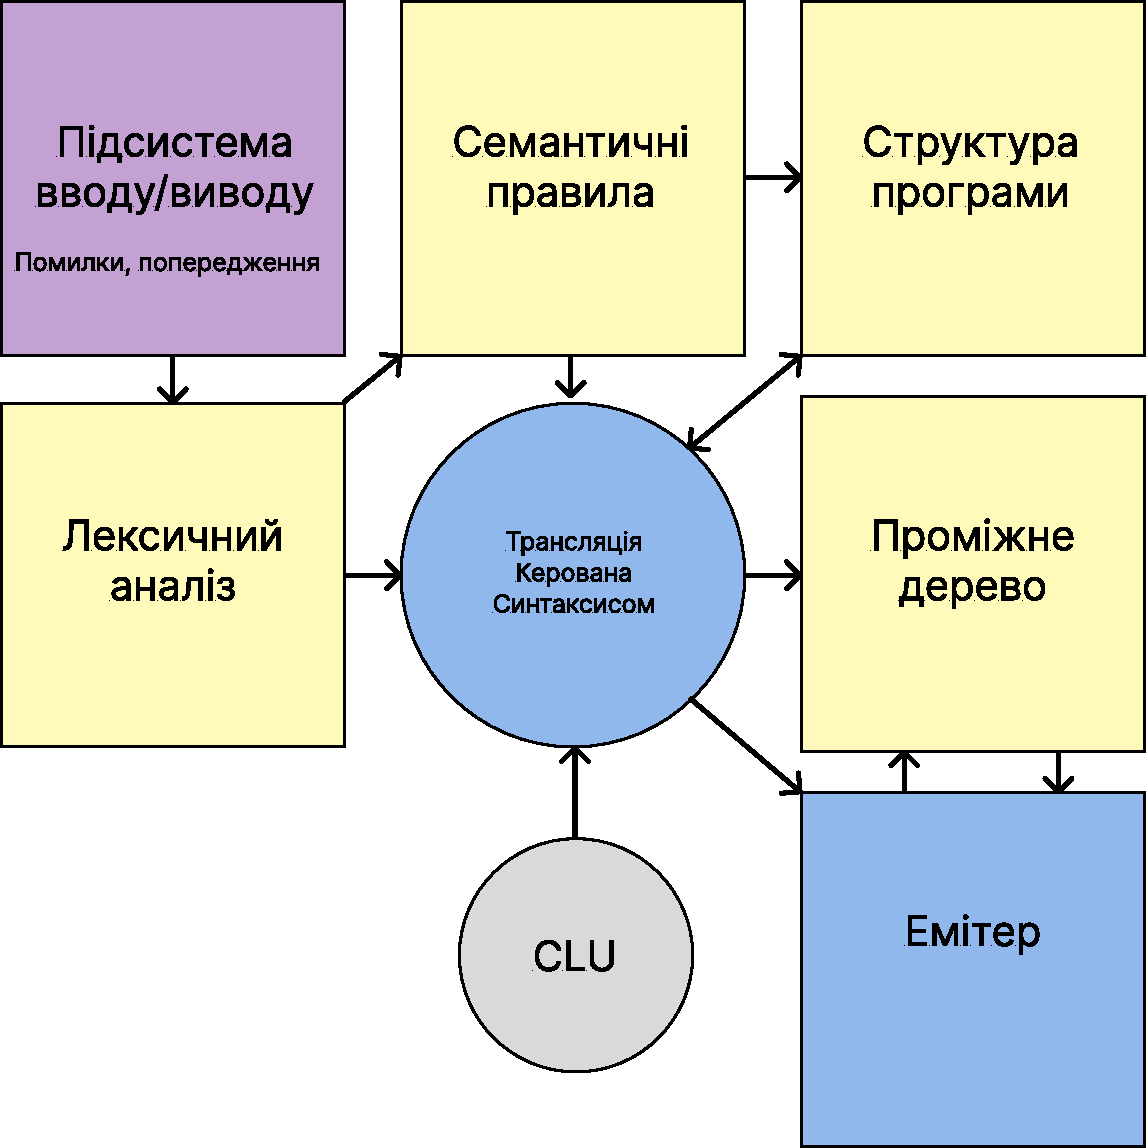
\includegraphics[scale=0.4,page=1]{pl1.pdf}};
\end{tikzpicture}

\section{Підсистема вводу/виводу}

Завдяки уніфікованому інтерфейсу підсистеми введення виведення IOS можна легко змінювати способи повідомлень про помилки та попередження компілятора.

Наслідуючи інтерфейс IIoSubsystem, реалізовано дві підсистеми – одна для консольних додатків, друга для віконної середовища GUI, яка інформує в окремому вікні про виявлені помилки компілятора.

\newpage
\section{Алфавіт мови}
Лексичний аналізатор LEX обробляє коментарі, числові константи, ідентифікатори та виконує пошук ідентифікаторів. Односимвольні термінали:

\begin{lstlisting}
\$	=	-	+	*	/	'	:
;	.	,	(	)	%	&	^
#	|	!	>	<	~	`	\
]	[	}	{	"	?	_
\end{lstlisting}

Двосимвольні термінали:

\begin{lstlisting}
<=	**	>=	!=
	->	/*	*/	!<
!>	||	..
\end{lstlisting}

Операції-мнемоніки:
\begin{lstlisting}
GT   	LT   	GE   	LE   
NG   	NL   	NE   	EQU  
CAT  	PT   	NOT  	OR   
AND  	XOR  	MOD  	DIV  
MUL  	PLUS 	MINUS
\end{lstlisting}

Ключові слова:

\begin{lstlisting}
ASSIGN   	BY       
CALL     	DECLARE  
DCL      	DO       
ELSE     	END      
GO       	GOTO     
IF       	INITIAL  
LABEL    	LITERALLY
OPTIONS  	PROCEDURE
PROC     	RECURSIVE
RETURNS  	RETURN   
THEN     	TO       
WHILE    	CASE

BINARY		DECIMAL
FIXED		FLOAT
REAL			COMPLEX
VOID
\end{lstlisting}

\newpage
\section{Граматика мови}
Граматика без лівої рекурсії базується на граматиці мови MyC
із прикладів Microsoft Visual Studio .NET, модифікованій для PL/1:

\begin{lstlisting}
letter			::= "A-Za-z";
digit 			::= "0-9";
name 			::= letter { letter | digit };
integer 		::= digit { digit };
ident 			::= name | label;
factor 			::= (ident | integer | "(" expr ")" );
unary_factor 		::= ["+"|"-"] factor;
term1 			::= ["*"|"/"] factor;
term0 			::= factor { term1 };
first_term 		::= unary_factor term1;
math_expr 		::= first_term { ["+"|"-"] term0 }
rel_expr 		::= math_expr ("=="|"!="|"<"|">"|">="|"<=") math_expr;
not_factor 		::= ["!"] rel_expr;
term_bool 		::= not_factor { ("&" | "&&") not_factor };
bool_expr 		::= term_bool { ("|" | "^") term_bool };
expr 			::= bool_expr;
var 			::= ident;
var_list 		::= var { "," var_list };
assign_stmt 		::= var_list "=" expr;
param 			::= "(" var_list ")";
declare 		::= ( "dcl" | "declare" ) "(" var | param ")" { "(" integer ")" } type;
type			::= "fixed"|"binary"|"float"|"decimal" ;
if_stmt 		::= "if" expr "then" stmt [ "else" stmt;
do_stmt 		::= "do" (null_stmt  smtm; | "while" expr null_stmt stmt
                          | assign_stmt  "to" expt null_stmt stmt) "end" null_stmt
rets_stmt		::= "returns" "(" type ")";
proc_decl 		::= ident ":" proc ;
proc 			::= param ["recursive"][ rets_stmt ] null_stmt stmt { stmt } "end" ident  null_stmt ;
goto_stmt 		::= ("go to" | "goto" ) ( ident | integer ) null_stmt;
ident_stmt 		::= (ident "=" expr| ident ":" stmt | ident { , ident } = expr) null_stmt;
ret_stmt 		::= "return" [ expr ] ";";
null_stmt 		::= ";";
stmt 			::= (ret_stmt null_stmt | ident_stmt | do_stmt null_stmt | goto_stmt null_stmt
                          | proc_decl null_stmt | decl_stmt null_stmt | if_stmt );
program_stmt  		::= stmt { stmt };
\end{lstlisting}

Завдяки виключенню лівої рекурсії, ця граматика фактично автоматично генерує
правила для написання процедур рекурсивного спуску для розбору. Усі підпрограми
рекурсивного спуску в модулі SYN складають основу синтаксично керованого
перетворення PL/IL, якщо вам потрібно розширити або доповнити синтаксис
мови, почніть саме тут.

\section{Опис мови}
\subsection{Ідентифікатори користувача}
Ідентифікатор обмежений 32 символами в довжину та повинен починатися з літерала,
може містити символи та цифри, а також знак долара, який ігнорується, коли
зустрічається в ідентифікаторі, тобто ідентифікатори first\$equation та
firstequation ідентичні (знак '\$' просто ігнорується компілятором і
використовується для зручності читання шляхом розділення вербальних
компонентів ідентифікатора). В PL/IL ідентифікатори не враховують регістр.

\subsection{Зарезервовані слова}
Зарезервовані слова завжди у верхньому регістрі:

\begin{lstlisting}
ASSIGN    BY   CALL DECLARE INITIAL   WHILE CASE
DCL       DO   ELSE END     GO GOTO   IF
LABEL     LITERALLY OPTIONS PROCEDURE PROC
RECURSIVE RETURNS   RETURN  THEN      TO
\end{lstlisting}

\subsection{Константи}
Числові константи в PL/IL починаються з цифри та можуть супроводжуватися
специфікатором: O та Q для вісімкових констант, H для шістнадцяткових, D
для десяткових та B для двійкових. За замовчуванням (якщо специфікатор
не вказано) використовується десятковий режим.

Комплексні константи, а також константи з плаваючою та фіксованою комою,
не підтримуються в PL/IL. Рядкові константи подібні до тих, що є в Паскалі.

\subsection{Операції у виразах}
\textbf{Сепаратори}. Вирази, що зустрічаються в операторах присвоєння,
а також в умовних конструкціях, таких як IF, WHILE, DO, можуть містити
роздільник "дужки" - ")", "(", які групують операнди за відомим принципом.
Інші типи роздільників будуть описані нижче.

PL/IL має 7 арифметичних операцій.

\begin{itemize}
\item + --- Оператор додавання.
\item - --- Оператор віднімання або унарний мінус.
\item PLUS --- Додавання з переносом.
\item MINUS --- Віднімання з переносом.
\item * --- Множення.
\item / --- Цілочисельне ділення.
\item MOD --- Залишок від ділення.
\end{itemize}

Шість реляційних конструкцій:

\begin{itemize}
\item < Менше ніж.
\item >= Більше ніж або дорівнює.
\item > Більше ніж.
\item <= Менше ніж або дорівнює.
\item = Дорівнює (точно той самий оператор присвоєння).
\item != Не дорівнює.
\end{itemize}

Логічні операції, дозволені у виразах, представлені чотирма зарезервованими словами:

\begin{itemize}
\item NOT Унарний логічний оператор заперечення.
\item AND Логічне множення.
\item OR Логічне додавання.
\item XOR Виключне "або".
\end{itemize}

Приклади конструкцій рідких виразів:

\begin{lstlisting}[mathescape=true]
IF ((4D > 5 * (-2AH) / (-5+7)) & (6 < 9)) THEN ;
IF (4O > 5) | (6 < 9H) | (9O = 0P) THEN ;
A, B, C = 50 * 50 * ( 5 + 5 * (-1) * 2 * ( 3H + 0ABH ) )
\end{lstlisting}

\subsection{Пріоритети операцій}
\begin{enumerate}
    \item \( *, /, \text{MOD} \)
    \item \( +, -, \text{PLUS}, \text{MINUS} \)
    \item \( <, <=, =, =>, >, != \)
    \item \( \text{NOT} \)
    \item \( \text{AND} \)
    \item \( \text{OR}, \text{XOR} \)
\end{enumerate}

\subsection{Мовні конструкції}
Приклади:
\begin{lstlisting}
IF ((4D > 5 * (-2AH) / (-5+7)) & (6 < 9)) THEN ;
DO WHILE expression; { statement; } END;
\end{lstlisting}

\section{Емітер}
Підсистема генерації коду EMT має модульну архітектуру. Під час контекстно-керованого емітінгу будується дерево виведення IAsm, яке використовується для генерації об’єктного коду.

\section{Повідомлення компілятора}

Помилки синтаксичного аналізатору (SYN):

\begin{itemize}
\item PL0101: invalid typecast (float to int)
\item PL0102: invalid typecast (long int to short int)
\item PL0103: invalid typecast (long float to short float)
\item PL0104: ')' expected.
\item PL0104: Using void function where expecting a value
\item PL0105: undeclared variable
\item PL0106: ')' expected
\item PL0107: invalid variable declaration
\item PL0108: ',' or ')' expected
\item PL0109: ident expected
\item PL0107: invalid variable declaration
\item PL0110: ')' expected
\item PL0111: invalid label declaration
\item PL0112: ':' expected
\item PL0107: invalid variable declaration
\item PL0113: constant expected
\item PL0114: ')' expected
\item PL0107: invalid variable declaration
\item PL0115: type specifier expected
\item PL0116: PROC declaration needs LABEL
\item PL0117: undeclared parameter
\item PL0118: END expected
\item PL0119: unclosed PROC
\item PL0120: invalid procedure declaration
\item PL0121: '=' expected
\item PL0122: undeclared variable
\item PL0123: TO expected
\item PL0124: END expected
\item PL0125: TO expected
\item PL0126: undefined label
\item PL0127: GOTO without direction
\item PL0128: illegal RETURN to nowhere
\item PL0129: ';' expected
\item PL0130: THEN expected
\item PL0131: ident after CALL expected
\item PL0132: invalid procedure call: undefined procedure
\item PL0133: invalid procedure call: not a procedure
\item PL0134: '(' expected
\item PL0135: ')' expected
\item PL0136: invalid procedure call: wrong number of parametrs
\item PL0137: undeclared variable
\item PL0137: undeclared variable
\item PL0138: ',' or '=' expected
\item PL0139: ident expected
\item PL0137: undeclared variable
\item PL0140: not found expected token ':', ',' or '='
\item PL0141: ';' expected
\item PL0142: expected statement but end of file encountered
\item PL0143: wild declaration found
\item PL0144: unknown construction
\item PL0145: wild symbol found
\end{itemize}

Помилки лексического анализатору (LEX):

\begin{itemize}
\item PL0201: invalid octal constant
\item PL0202: invalid decimal constant
\item PL0203: invalid binary constant
\item PL0204: invalid decimal constant
\end{itemize}

Помилки підсистеми емітінгу (EMT):

\begin{itemize}
\item PL0301: inhandled instruction type
\item PL0302: Unhandled instruction type
\end{itemize}

Помилки генератора лістінгів (ASM):

\begin{itemize}
\item PL0401: unhandled type
\item PL0402: load instruction with no variable ptr
\item PL0403: instruction load of unknown class ( classid )
\item PL0404: store instruction with no variable ptr
\item PL0405: instruction load of unknown class ( classid )
\item PL0406: could not find type for local
\item PL0407: unhandled field def type
\end{itemize}

Помилки генератора коду (EXE):

\begin{itemize}
\item ICE: unhandled type
\item ICE: load instruction with no variable ptr
\item ICE: instruction load of unknown class ( classid+)
\item ICE: store instruction with no variable ptr
\item ICE: instruction load of unknown class ( classid+)
\item ICE: no previous extern for
\item ICE: instruction opcode not found in hash
\item ICE: instruction branch opcode not found in hash
\item ICE: could not find opcode
\end{itemize}

\section{Автоматичне приведення скалярних типів}
\begin{table}[h]
    \centering
    \caption{Приведення типів при цілочисельних операціях}
    \begin{tabular}{|c|c|c|c|c|c|}
        \hline
        & Int16 & Int32 & Int64 & Float & double \\
        \hline
        Int16 & Int16 & Int32 & Int64 & Float & double \\
        Int32 & Int32 & Int64 & Int64 & Float & double \\
        Int64 & Int64 & Int64 & Int64 & float & double \\
        Float & float & float & float & Float & double \\
        double & double & double & double & double & double \\
        \hline
    \end{tabular}
\end{table}

\section{Бібліотека вбудованих функцій}
За допомогою бібліотеки вбудованих функцій LIB можна визначати та звертатися до відомих функцій .NET Framework безпосередньо, обминаючи громіздкі виклики через Reflection.

Ви можете розширювати та доповнювати існуючий набір функцій, що видно через систему типів PL/IL.

Приклади бібліотечних функцій:
\texttt{System.Console.WriteLine},
\texttt{System.Console.ReadLine}.

\section{Виклики Reflection}

За допомогою потужного механізму відображення ви можете викликати
будь-який метод будь-якого типу, що належить будь-якій збірці.
(Очікується у наступній версії PL/IL).

\section{Асемблер}
Для детального ознайомлення з набором CLI пропонуємо звернутися до стандартів ECMA,
які поставляються безкоштовно з Microsoft Visual Studio .NET.

\begin{lstlisting}
0x00	nop		0x01	break
0x02	ldarg.0		0x03	ldarg.1
0x04	ldarg.2		0x05	ldarg.3
0x06	ldloc.0		0x07	ldloc.1
0x08	ldloc.2		0x09	ldloc.3
0x0a	stloc.0		0x0b	stloc.1
0x0c	stloc.2		0x0d	stloc.3
0x0e	ldarg.s		0x0f	ldarga.s
0x10	starg.s		0x11	ldloc.s
0x12	ldloca.s	0x13	stloc.s
0x14	ldnull		0x15	ldc.i4.m1
0x16	ldc.i4.0	0x17	ldc.i4.1
0x18	ldc.i4.2	0x19	ldc.i4.3
0x1a	ldc.i4.4	0x1b	ldc.i4.5
0x1c	ldc.i4.6	0x1d	ldc.i4.7
0x1e	ldc.i4.8	0x1f	ldc.i4.s
0x20	ldc.i4		0x21	ldc.i8
0x22	ldc.r4		0x23	ldc.r8
0x25	dup		0x26	pop
0x27	jmp		0x28	call
0x29	calli		0x2a	ret
0x2b	br.s		0x2c	brfalse.s
0x2d	brtrue.s	0x2e	beq.s
0x2f	bge.s		0x30	bgt.s
0x31	ble.s		0x32	blt.s
0x33	bne.un.s	0x34	bge.un.s
0x35	bgt.un.s	0x36	ble.un.s
0x37	blt.un.s	0x38	br
0x39	brfalse		0x3a	brtrue
0x3b	beq		0x3c	bge
0x3d	bgt		0x3e	ble
0x3f	blt		0x40	bne.un
0x41	bge.un		0x42	bgt.un
0x43	ble.un		0x44	blt.un
0x45	switch		0x46	ldind.i1
0x47	ldind.u1	0x48	ldind.i2
0x49	ldind.u2	0x4a	ldind.i4
0x4b	ldind.u4	0x4c	ldind.i8
0x4d	ldind.i		0x4e	ldind.r4
0x4f	ldind.r8	0x50	ldind.ref
0x51	stind.ref	0x52	stind.i1
0x53	stind.i2	0x54	stind.i4
0x55	stind.i8	0x56	stind.r4
0x57	stind.r8	0x58	add
0x59	sub		0x5a	mul
0x5b	div		0x5c	div.un
0x5d	rem		0x5e	rem.un
0x5f	and		0x60	or
0x61	xor		0x62	shl
0x63	shr		0x64	shr.un
0x65	neg		0x66	not
0x67	conv.i1		0x68	conv.i2
0x69	conv.i4		0x6a	conv.i8
0x6b	conv.r4		0x6c	conv.r8
0x6d	conv.u4		0x6e	conv.u8
0x6f	callvirt	0x70	cpobj
0x71	ldobj		0x72	ldstr
0x73	newobj		0x74	castclass
0x75	isinst		0x76	conv.r.un
0x79	unbox		0x7a	throw
0x7b	ldfld		0x7c	ldflda
0x7d	stfld		0x7e	ldsfld
0x7f	ldsflda		0x80	stsfld
0x81	stobj		0x82	conv.ovf.i1.un
0x83	conv.ovf.i2.un	0x84	conv.ovf.i4.un
0x85	conv.ovf.i8.un	0x86	conv.ovf.u1.un
0x87	conv.ovf.u2.un	0x88	conv.ovf.u4.un
0x89	conv.ovf.u8.un	0x8a	conv.ovf.i.un
0x8b	conv.ovf.u.un	0x8c	box
0x8d	newarr		0x8e	ldlen
0x8f	ldelema		0x90	ldelem.i1
0x91	ldelem.u1	0x92	ldelem.i2
0x93	ldelem.u2	0x94	ldelem.i4
0x95	ldelem.u4	0x96	ldelem.i8
0x97	ldelem.i	0x98	ldelem.r4
0x99	ldelem.r8	0x9a	ldelem.ref
0x9b	stelem.i	0x9c	stelem.i1
0x9d	stelem.i2	0x9e	stelem.i4
0x9f	stelem.i8	0xa0	stelem.r4
0xa1	stelem.r8	0xa2	stelem.ref
0xb3	conv.ovf.i1	0xb4	conv.ovf.u1
0xb5	conv.ovf.i2	0xb6	conv.ovf.u2
0xb7	conv.ovf.i4	0xb8	conv.ovf.u4
0xb9	conv.ovf.i8	0xba	conv.ovf.u8
0xc2	refanyval	0xc3	ckfinite
0xc6	mkrefany	0xd0	ldtoken
0xd1	conv.u2		0xd2	conv.u1
0xd3	conv.i		0xd4	conv.ovf.i
0xd5	conv.ovf.u	0xd6	add.ovf
0xd7	add.ovf.un	0xd8	mul.ovf
0xd9	mul.ovf.un	0xda	sub.ovf
0xdb	sub.ovf.un	0xdc	endfinally
0xdd	leave		0xde	leave.s
0xdf	stind.i		0xe0	conv.u

0xfe 0x00	arglist		0xfe 0x01	ceq
0xfe 0x02	cgt		0xfe 0x03	cgt.un
0xfe 0x04	clt		0xfe 0x05	clt.un
0xfe 0x06	ldftn		0xfe 0x07	ldvirtftn
0xfe 0x09	ldarg		0xfe 0x0a	ldarga
0xfe 0x0b	starg		0xfe 0x0c	ldloc
0xfe 0x0d	ldloca		0xfe 0x0e	stloc
0xfe 0x0f	localloc	0xfe 0x11	endfilter
0xfe 0x12	unaligned.	0xfe 0x13	volatile.
0xfe 0x14	tail.		0xfe 0x15	initobj
0xfe 0x17	cpblk		0xfe 0x18	initblk
0xfe 0x1a	rethrow		0xfe 0x1c	sizeof
0xfe 0x1d	refanytype
\end{lstlisting}

Насправді ми не використовували всі можливості CLR/CLI. Більше того,
всі константи операцій визначено в Reflection.Emit, тут ми просто показали
повний набір операцій, які надає нам наше середовище.

\chapter{Апробація}
\section{Системи автоматичного тестування}
Для перевірки стабільності використано систему NUNIT.

\section{Розробка штурмових тестів}
Більшість часу на розробку стабільного компілятора витрачається на
підготовку штурмових тестів. Автори PL/IL особливо ретельно розробили
підхід до написання прикладів PL/IL програм.

\subsection{Приклад 1}

\begin{lstlisting}
Main: PROC;
    DCL ( P1, P2, P3 ) FIXED;
    P1 = 1Ah;
    P2 = 1001b;
    P3 = 150;
    CALL PRINT_I(P1);
    CALL PRINT_I(P2);
    CALL PRINT_I(P3);
END Main;
\end{lstlisting}

\begin{lstlisting}
.assembly 'test1'
{
.ver 0:0:0:0
}

.class test1 {
.method public static void Main() {
.entrypoint
.locals (int32,int32,int32,int32)
L@@Main:
ldc.i4.s 26 	//1
stloc 0		//2, P1
ldc.i4.s 9		//3
stloc 1		//4, P2
ldc/i4 150 //5
stloc 2
		//6, P3
ldloc 0		//7, P1
call void [mscorlib]System.Console::WriteLine(int32) //8
ldloc 1		//9, P2
call void [mscorlib]System.Console::WriteLine(int32) //10
ldloc 2		//11, P3
call void [mscorlib]System.Console::WriteLine(int32) //12
ret			//13
}
}
\end{lstlisting}

\subsection{Приклад 2}

\begin{lstlisting}
MAIN1:	PROC ( X, Y, Z );
DCL ( X, Y, Z ) FIXED;
    	DCL A1 FIXED;
    	DCL A2 FIXED;
		A2 = -3;
		Z = A2 + 5*X - Y;
    	IF A1 >= Z THEN A1 = Z;
END 	MAIN1;

Main: 	PROC;
END 	Main;
\end{lstlisting}

\begin{lstlisting}
.assembly 'test2'
{
.ver 0:0:0:0
}

.class test2 {
		.method public static void MAIN1(int32,int32,int32) {
		.locals (int32,int32)
L@@MAIN1:
		ldc.i4.s -3		//1
		stloc 1		//2, A2
		ldloc 1		//3, A2
		ldc.i4.5		//4
		ldarg 0		//5, X
		mul			//6
		add			//7
		ldarg 1		//8, Y
		sub			//9
		starg 2		//10, Z
		ldloc 0		//11, A1
		ldarg 2		//12, Z
		clt			//13
		ldc.i4.0		//14
		ceq			//15
		brfalse L@@0	//16
		ldarg 2		//17, Z
		stloc 0		//18, A1
L@@0:
		ret			//19
}

.method public static void Main() {
.entrypoint
.locals ()
L@@Main:
ret			//1
		}
}
\end{lstlisting}

\subsection{Приклад 3}

\begin{lstlisting}
Main:   PROC;
        DCL ( Y, A, B ) FIXED;
        DO WHILE 4 > 6;
           Y = 1;
        END;
ZZZ:    A = 33;
        A, B, Y = 7+4-5;
        B = 2H;
        GOTO ZZZ;
END     Main;
\end{lstlisting}

\begin{lstlisting}
.assembly 'test3'
{
.ver 0:0:0:0
}

.class test3 {
.method public static void Main() {
.entrypoint
.locals (int32,int32,int32)
L@@Main:
L@@0:
		ldc.i4.4		//1
		ldc.i4.6		//2
		cgt			//3
		brfalse L@@1	//4
		ldc.i4.1		//5
		stloc 0		//6, Y
		br L@@0		//7
L@@1:
L@@ZZZ:
		ldc.i4.s 33		//8
		stloc 1		//9, A
		ldc.i4.7		//10
		ldc.i4.4		//11
		add			//12
		ldc.i4.5		//13
		sub			//14
		stloc 1		//15, A
		ldloc 1		//16, A
		stloc 2		//17, B
		ldloc 1		//18, A
		stloc 0		//19, Y
		ldc.i4.2		//20
		stloc 2		//21, B
		br L@@ZZZ		//22
		ret			//23
		}
}
\end{lstlisting}

\subsection{Приклад 4}

\begin{lstlisting}
Main:   PROC;
        DCL B FIXED;
        B = 2H;
        B = 1BH;
        B = 1B;
        B = 7O;
END     Main;
\end{lstlisting}

\begin{lstlisting}
.assembly 'test4'
{
.ver 0:0:0:0
}

.class test4 {
.method public static void Main() {
.entrypoint
.locals (int32)
L@@Main:
		ldc.i4.2		//1
		stloc 0		//2, B
		ldc.i4.s 27		//3
		stloc 0		//4, B
		ldc.i4.1		//5
		stloc 0		//6, B
		ldc.i4.7		//7
		stloc 0		//8, B
		ret			//9
		}
}
\end{lstlisting}

\subsection{Приклад 5}

\begin{lstlisting}
SUM:    PROC ( X1, Y1 );
        DCL ( X1, Y1 ) FIXED;
        DCL R FIXED;
        R = X1 + Y1;
END     SUM;

Main:   PROC;
        DCL ( P1, P2, P3 ) FIXED;
        DCL F FLOAT;
        DCL C COMPLEX;
        DCL D FIXED;
        P1, P2, P3 = -2*4;
        P1 = F + C;
        CALL SUM(P1, P2);
END     Main;
\end{lstlisting}

\begin{lstlisting}
.assembly 'test7'
{
.ver 0:0:0:0
}

.class test7 {
.method public static void SUM(int32,int32) {
		.locals (int32)
L@@SUM:
		ldarg 0		//1, X1
		ldarg 1		//2, Y1
		add			//3
		stloc 0		//4, R
		ret			//5
		}

		.method public static void SUMFLT(float64,float64) {
		.locals (float64)
L@@SUMFLT:
		ldarg 0		//1, X1
		ldarg 1		//2, Y1
		add			//3
		stloc 0		//4, R
		ret			//5
		}
	
.method public static void Main() {
		.entrypoint
		.locals (int32,int32,int32,float32,float64,int32)
L@@Main:
		ldc.i4.s -2		//1
		ldc.i4.4		//2
		mul			//3
		stloc 0		//4, P1
		ldloc 0		//5, P1
		stloc 1		//6, P2
		ldloc 0		//7, P1
		stloc 2		//8, P3
		ldc.i4.s -5		//9
		stloc 4		//10, C
		ldc.i4.s 17		//11
		stloc 0		//12, P1
		ldloc 0		//13, P1
		ldloc 4		//14, C
		call void test7::SUMFLT(float64,float64)					//15
		ret			//16
		}
}
\end{lstlisting}

\subsection{Приклад 6}

\begin{lstlisting}
HANOY:	PROC ( N, SRC, DST, MID );
		DCL (N, SRC, DST, MID) FIXED;
		IF N > 0 THEN DO;
			CALL HANOY(N - 1, SRC, MID, DST);
			CALL PRINT_I ( N );
			CALL PRINT_I ( SRC );
			CALL PRINT_I ( DST );
			CALL PRINT_I ( MID );
			CALL PRINT_I ( 0 );
			CALL HANOY(N - 1, MID, DST, SRC);
		END;
END	HANOY;

Main:	PROC;
		CALL HANOY(3, 1, 3, 2);
END	Main;
\end{lstlisting}

\begin{lstlisting}
.assembly 'hanoy'
{
		.ver 0:0:0:0
}

.class hanoy {
.method public static void HANOY(int32,int32,int32,int32) {
		.locals ()
L@@HANOY:
		ldarg 0		//1, N
		ldc.i4.0		//2
		cgt			//3
		brfalse L@@0	//4
		ldarg 0		//5, N
		ldc.i4.1		//6
		sub			//7
		ldarg 1		//8, SRC
		ldarg 3		//9, MID
		ldarg 2		//10, DST
		call void hanoy::HANOY(int32,int32,int32,int32) //11
		ldarg 0		//12, N
		call void [mscorlib]System.Console::WriteLine(int32)	//13
		ldarg 1		//14, SRC
		call void [mscorlib]System.Console::WriteLine(int32)	//15
		ldarg 2		//16, DST
		call void [mscorlib]System.Console::WriteLine(int32)	//17
		ldarg 3		//18, MID
		call void [mscorlib]System.Console::WriteLine(int32)	//19
		ldc.i4.0		//20
		call void [mscorlib]System.Console::WriteLine(int32)	//21
		ldarg 0		//22, N
		ldc.i4.1		//23
		sub			//24
		ldarg 3		//25, MID
		ldarg 2		//26, DST
		ldarg 1		//27, SRC
		call void hanoy::HANOY(int32,int32,int32,int32)	 //28
		br L@@0		//29
L@@2:
L@@0:
		ret			//30
		}

		.method public static void Main() {
		.entrypoint
		.locals ()
L@@Main:
		ldc.i4.3		//1
		ldc.i4.1		//2
		ldc.i4.3		//3
		ldc.i4.2		//4
		call void hanoy::HANOY(int32,int32,int32,int32)	 //5
		ret			//6
		}
}
\end{lstlisting}

\section{Висновки}
Як бачите, використовуючи настільки потужні сучасні засоби розробки, реалізація
такого складного програмного продукту, як компілятор, не складає особливих труднощів.
Заради справедливості, хочеться відзначити, що реалізація подібної витівки на
Java, або, більше того, на C, видалася б не особливо привабливою.

Дякуємо науковим керівникам та розробникам Microsoft за технічні засоби.

\begin{thebibliography}{99}

\bibitem{FrolovOlyunin} Фролов Г.\,Д., Олюнин В.\,Ю. \textit{Практический курс программирования ПЛ/1}.
\bibitem{BukhtiyarovEtAl} Бухтияров А.\,М., Фролов Г.\,Д., Олюнин В.\,Ю. \textit{Сборник задач программирования на языке ПЛ/1}.
\bibitem{Aho} Ахо А.\,В., Сети Р., Ульман Д.\,Д. \textit{Компиляторы: принципы, технологии и инструменты}.
\bibitem{Knuth} Кнут Д.\,Э. \textit{Искусство программирования.} В 3 томах.
\bibitem{XPL} Маккиман Дж., Хорнинг Дж.\,Д., Уортман Б.\,А. \textit{Генератор компиляторов. Описание XPL}.
\bibitem{Rossoshinskiy} Россошинский Д.\,А. \textit{Конспект лекций}, 2003--2004.
\bibitem{Petzold} Петцольд Ч. \textit{Программирование на C\# для Windows.} В 2 томах.
\bibitem{MSDN} Microsoft. \textit{MSDN}, апрель 2003.

\end{thebibliography}

\end{document}
